\chapter{Editing: real-world usage cases}%
\label{cha:editing_real_world_usage}

\section{Workflow with OpenEDL and Nested Clips\protect\footnote{credit fary54}}%
\label{sec:workflow_openedl_nested_clips}

This is a real world usage case that provides an excellent example of how OpenEDL has been a
revolution for \CGG{}. Advantages include: editing speed, clarity, ease of finding a specific item,
and movement of a subject block via \textit{Nest to media}.
The main concept of editing using OpenEDL in this real world case is to
reduce a large quantity of videos and shots to a few big clips by using
an OpenEDL session for each clip. Using the OpenEDL timeline is similar to
 using the normal timeline: you can add effects, cut and drag, add or delete
tracks, etc.

For more information on OpenEDL and Nested clips see sections \nameref{sub:edit-edls} and \nameref{sub:nesting}.

Scenario setup consists of making one hour videos using 3 different cameras:

\begin{itemize}
	\item \textit{Footage 1:} A person uses camera 1 to shoot a general view of the subject (e.g. a jazz group concert).
	\item \textit{Footage 2:} Another person uses camera 2 to film a detail of a specific subject (e.g. saxophonist or trumpet player).
	\item \textit{Footage 3:} Contains images of the journey between the subjects (action cam on the windshield of a moving car, on the helmet of a biker, on the handlebars of a bicycle, or on a boat).
\end{itemize}

\textit{Note:} Camera 1 and 2 are both filming the same subject so the number of hours for the footage from these two cameras easily reaches 20 hours, but the final movie can only be one hour maximum.  For this case, the final movie consists of all the subjects separated by camera 3 footage.

\textit{Workflow:} OpenEDL is used throughout the editing process with the timeline reserved as the workspace. Basically, every time you have to work on a clip (consisting of one or more tracks), you use OpenEDL instead of the classic method of bringing each clip to the timeline, before doing the necessary Drag and Drop or Cut and Paste operations between different tracks. When finished with each
OpenEDL clip session, save it outside of the OpenEDL layer at the top level of the main timeline.

See \href{https://youtu.be/0li5DdeQ6_o}{Video 1} (using French locale).


\subsubsection*{Pre-sorting of the footage}
\label{ssub:pre_sorting_footage}

	\begin{itemize}
		\item Load all the shots from camera 1 and create a single clip; do the same with cameras 2 and 3.
		\item Watch each clip and sort the images to keep (via OpenEDL); delete the blurred footage and the images you do not want to keep.
	\end{itemize}

\begin{figure}[htpb]
	\centering
	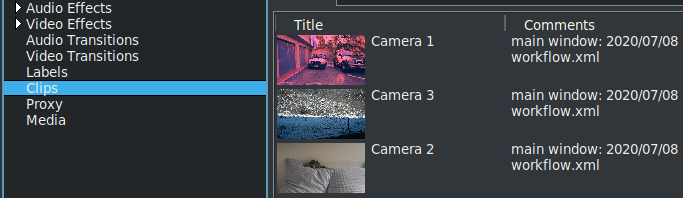
\includegraphics[width=0.8\linewidth]{openedl-01.png}
	\caption{three clips modified with OpenEDL}
	\label{fig:openedl-01}
\end{figure}

\textit{Camera 1} contains shots of Barcelona and Lisbon concert made by Camera 1.

\textit{Camera 2} contains shots of Barcelona and Lisbon concert made by Camera 2.

\textit{Camera 3} contains the images of the journey between the first subject and the second (e.g from Barcelona to Lisbon).

\subsubsection*{Extraction of the subjects}
\label{ssub:extraction_subjects}

Next extract each common subject from the camera 1 \& 2 footage and create a clip, for example - a place, a city, or a subject. In this case scenario, it is a concert in a specific city.
You end up with as many clips as there are subjects (e.g. Barcelona \& Lisbon).
 See figure ~\ref{fig:openedl-02}.

\begin{figure}[htpb]
	\centering
	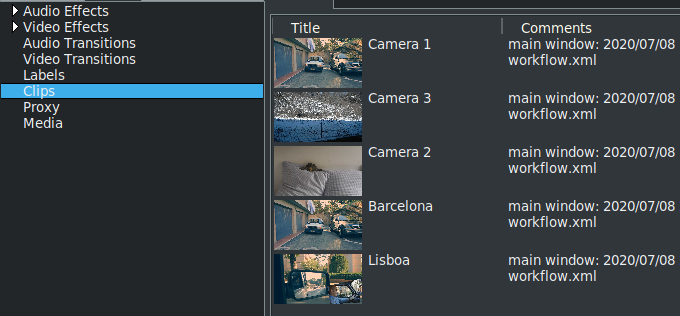
\includegraphics[width=0.8\linewidth]{openedl-02.png}
	\caption{a new clip for each subject: Barcelona and Lisbon}
	\label{fig:openedl-02}
\end{figure}

Each subject selected contains 2 video tracks and 4 audio tracks. See figure ~\ref{fig:openedl-03} of a Barcelona clip.

\begin{figure}[htpb]
	\centering
	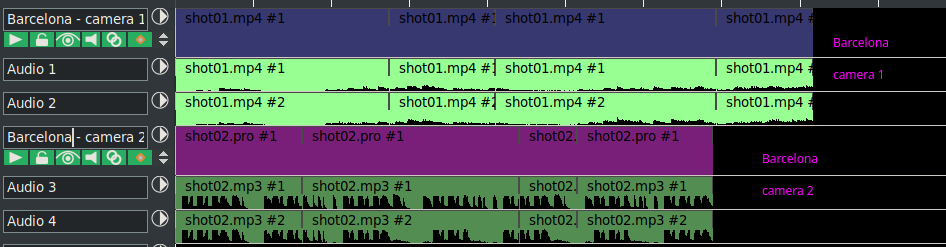
\includegraphics[width=1.0\linewidth]{openedl-03.png}
	\caption{Barcelona clip: 2 video tracks and 4 audio tracks}
	\label{fig:openedl-03}
\end{figure}

\subsubsection*{Editing of the subjects}
\label{ssub:editing_subjects}

Then edit each subject via OpenEDL. From the 2 tracks 1 \& 4 (camera 1 \& 2) you create a a single track (+ 2 audio tracks) as seen in figure ~\ref{fig:openedl-04}.

\begin{figure}[htpb]
	\centering
	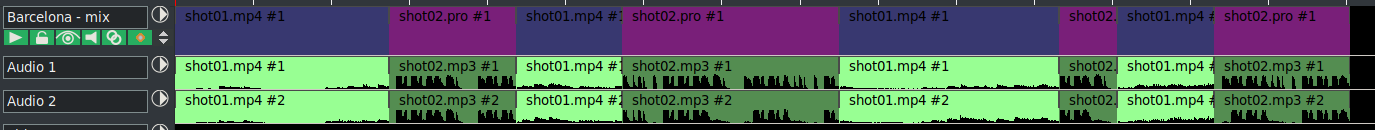
\includegraphics[width=1.0\linewidth]{openedl-04.png}
	\caption{Barcelona clip: 2 video tracks to 1 video track}
	\label{fig:openedl-04}
\end{figure}

\subsubsection*{Add sound effects and video/audio effects}
\label{ssub:add_sound_video_effects}

Next add the sound effects (such as birds or a water fountain) and video / audio effects for each subject; again via OpenEDL.

\subsubsection*{Compaction}
\label{ssub:compaction}

Each subject is converted to a nested clip by using the \textit{Nest to media} option, making it a group.

\begin{figure}[htpb]
	\centering
	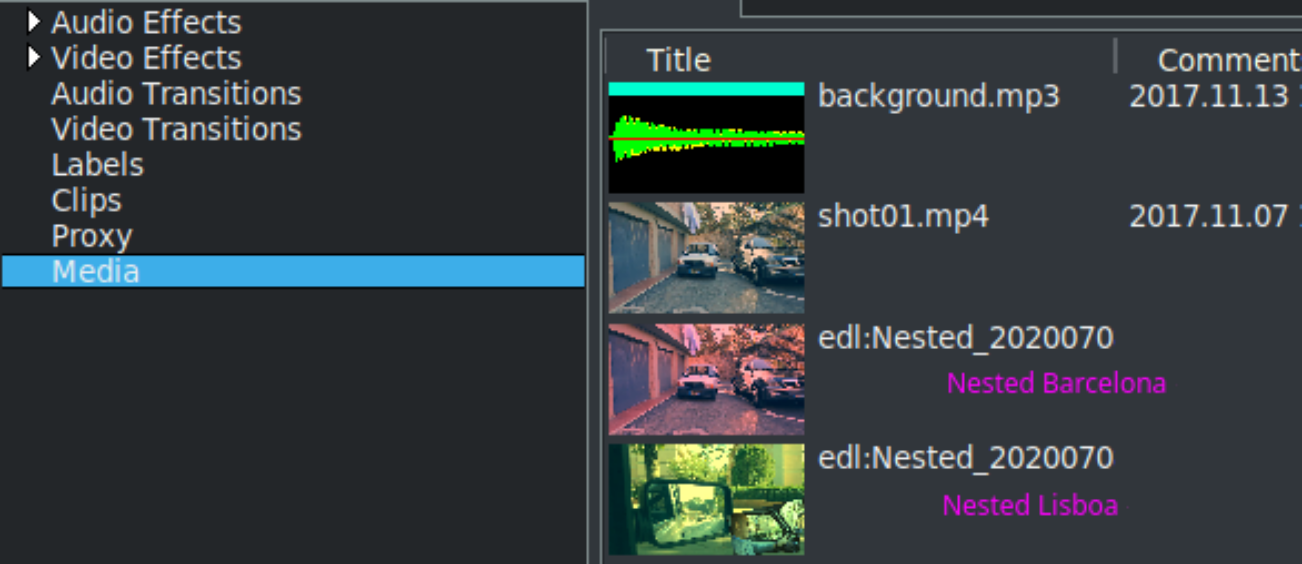
\includegraphics[width=0.8\linewidth]{openedl-05.png}
	\caption{two new nested clips: Barcelona and Lisbon}
	\label{fig:openedl-05}
\end{figure}

The subject converted to a nested clip is automatically moved from the Clip folder to the Media folder.

See \href{https://youtu.be/kQ7sGq0o44U}{Video 2} (using French locale).

\subsubsection*{Final assembly}
\label{ssub:final_assembly}

Import each subject (Nested clip) on the main timeline. Converting using Nest to Media makes it easy to move and position each subject. You can move one subject after or before another.

\begin{figure}[htpb]
	\centering
	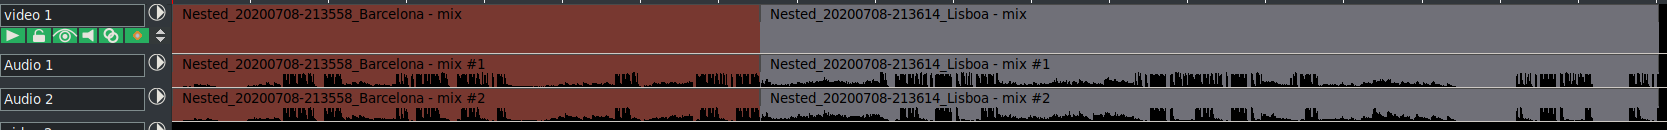
\includegraphics[width=1.0\linewidth]{openedl-06.png}
	\caption{Barcelona and Lisbon nested clips on timeline}
	\label{fig:openedl-06}
\end{figure}

Insert the retained shots coming from \textit{camera 3} between the different subjects.

\begin{figure}[htpb]
	\centering
	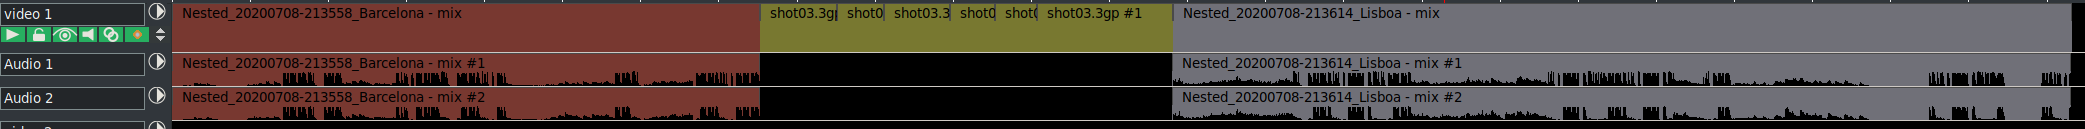
\includegraphics[width=1.0\linewidth]{openedl-07.png}
	\caption{camera 3 footage between Barcelona and Lisbon nested clips}
	\label{fig:openedl-07}
\end{figure}

See \href{https://youtu.be/9Hz0a-1i3I8}{Video 3} (using French locale).

Add background music and comments.

\begin{figure}[htpb]
	\centering
	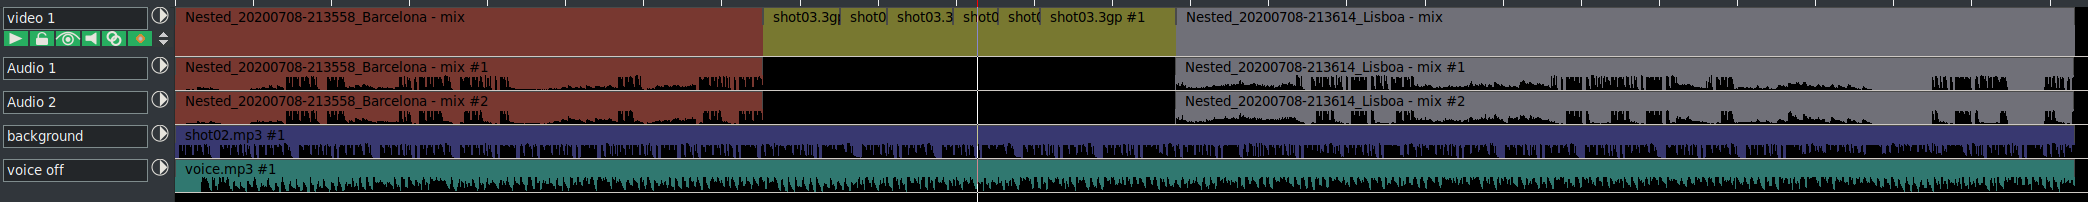
\includegraphics[width=1.0\linewidth]{openedl-08.png}
	\caption{completion of the work}
	\label{fig:openedl-08}
\end{figure}

\subsubsection*{More editing}
\label{ssub:more_editing}

At this stage, each subject can still be edited and undergo any modification via OpenEDL (again ... and always)

\subsubsection*{Render your movie}
\label{ssub:render_movie}

All that remains is mastering the video with a render.

Ordinarily it it is very difficult to set up such a project but using tools such as OpenEDL and Nested clips makes it quite easy. These tools, in many cases, are essential and become standards for the development of important projects using \CGG{}.

\subsubsection*{Important Notes}
\label{ssub:important_notes}

\begin{itemize}
	\item It is recommended that you save your project, not inside an OpenEDL, but rather after you exit openEDL and are on the main timeline.
	\item Once converted to nest to media the clips disappear from the clips folder to end up in the media folder. You can always, if you wish to recover it in the clips folder do so via the \textit{EDL to clip} menu. In this case, the name of the clip can change but the reference of the clip can be found in the comment of the clip.
\end{itemize}

See \href{https://youtu.be/bfYaBqVbdCo}{Video 4} (using French locale).
